\section{Example Experiments}
\label{sec-experiments}

During our first beta test year we performed a usage measurement study. 115
participants joined the study which eventually ran for over six months. For
this purpose, we have developed a measurement application that collects
multiple salient features of smartphone usage: networking, mobility, power
consumption, and application usage. This section presents some selected
results of this study. We present the battery and charging behavior first
then the network transition behavior between 3G and Wifi next. Our goal is to
demonstrate the types of experiments that can be performed on \PhoneLab{} and
the insights they can achieve.

\subsection{Energy Breakdown}
\label{subsec-energybreakdown}

A single-day component-by-component breakdown is shown in
Figure~\ref{figure-batteryoverview}. Our results are similar to those reported
by a previous smaller-scale study~\cite{shye:micro:2009}, and indicate that
mobile data (labeled as ``Idle data'' and ``Active data'' depending on the
state), the screen, and CPU usage are the main sources of smartphone power
consumption. The per-participant bars also show a great deal of variation, with
differences in both the amount and the breakdown of energy consumed by each
participant.

One supposedly power-hungry component that has less of an impact than we had
expected is the GPS. This is particularly surprising given the large amount
of location-monitoring work motivated by GPS power consumption. One of
several factors may be at work. First, the Android platform estimates the GPS
chipset current consumption at 50~mA. This number is used by the standard
``Fuel Gauge'' battery monitor and by our calculations. However, it is lower
than the data sheet for the Broadcom 4751 GPS receiver~\cite{bcm4751} and may
represent a best-case average. Still, even if the GPS current consumption is
off by as much as a factor of five, it does not represent a significant
contribution. Other hypotheses are that Android network location is providing
location with sufficient accuracy for many applications, eliminating the need
for GPS, or participants and applications may simply be conscious of GPS
power consumption and taking steps to control it.

\begin{figure}[htb!]

\centering
\includegraphics[width=0.75\columnwidth]{./figures/power/opportunistic_charging/count_and_by_time/graph.pdf}

\vspace*{-0.1in}

\caption{\textbf{Charging patterns.} Many users perform opportunistic
charging during the day, with habitual charging occurring at night.}

\label{fig-opportunistic-patterns}

\vspace*{0.1in}

\centering
\includegraphics[width=\columnwidth]{./figures/power/opportunistic_charging/max_difference/graph.pdf}

\caption{\textbf{Charge difference between participants during one day.} The
graph plots the top and bottom quartiles as well as the median. At any given
time, a significant spread is present.}

\label{fig-opportunistic-spread}

\vspace*{-0.4in}

\end{figure}

\subsection{Opportunistic Charging}
\label{subsec-opportunistic}

One way that users work around the battery limitations of their smartphone
devices is by finding new times and places to charge their phones: plugging
in at their desk at work, in the car during their commute, or at home before
a long night out. We refer to these charging sessions as
\textit{opportunistic} to distinguish them from \textit{habitual} nightly
charging. Assuming that many smartphone users encounter plug points
throughout the day, engaging in opportunistic charging becomes an additional
sign of energy awareness, and understanding opportunistic charging becomes
necessary to improving energy management on mobile devices. Others have analyzed
this behavior before~\cite{banerjee:ubicomp:2007, rahmati:mobilehci:2007} and
our goal is to examine the battery charging behavior of \PhoneLab{} participants.

Figure~\ref{fig-opportunistic-patterns} shows that many users engage in
opportunistic charging. We define a charging session as opportunistic if is
longer than 10~minutes but does not restore the battery to a fully-charged
state, indicating that the user disconnected the device before charging could
finish. For a representative day during our experiment, of the 245 charging
sessions we observed that day, 96 (39\%) were opportunistic by this
definition. 50 of 95 active participants engaged in opportunistic charging at
some point during our experiment an average of once per day.

Opportunistic charging may be a response to an anticipated need for more
smartphone battery power, as when a student plugs her smartphone in to charge
before a night out. Our data also allowed us to examine how many of these
opportunistic charging sessions were necessary to bridge the gap to the next
full charge. We found that 24 of the 96 (25\%) of the opportunistic charges
we observed were necessary. We believe that this indicates that participants
have responded to their smartphones' battery limitations by engaging in
conservative charging behavior, grabbing power whenever possible even if they
do not anticipate needing it later.

Opportunistic charging combined with the varied rhythms of our participants
creates a second interesting effect: at any given point there is a wide
disparity in the amount of power available on different phones.
Figure~\ref{fig-opportunistic-spread} displays the top, bottom, and middle
(median) quartiles for a single day on \PhoneLab{}. Only phones that are
discharging are shown, which explains the sharp increase between 6~and~10AM
as participants end nightly charging cycles.  As the graph indicates, it is
likely that when two smartphones meet they have very different battery
levels.

\subsection{Mobile Network Transitions}
\label{subsec-networktransitions}

Mobile smartphones move through a complex network environment. Providing the
illusion of seamless connectivity requires negotiating hand-offs both between
Wifi access points and between Wifi and 3G radios. We were interested in
observing hand-offs between 3G (provided by Sprint, \PhoneLab{}'s operational
partner) and Wifi and found many in the dataset collected by our usage
experiment. Since the Android \texttt{ConnectivityService} frequently
switches network interfaces for exploration purposes, we have defined a
transition as two one-minute or longer sessions on different interfaces
separated by less than one minute. We further limit ourselves to cases where
we received a location update during the transition. Data for the first
21~days of the usage experiment is shown.

\begin{figure*}[t]

\centering
\includegraphics[width=0.75\textwidth]{./figures/networking/transition_locations/graph.pdf}

\caption{\textbf{3G to Wifi transition locations.} The map indicates that
there are several common areas where network hand-offs occur.}

\label{figure-networktransitions}

\vspace*{-0.1in}

\end{figure*}

Figure~\ref{figure-networktransitions} plots the location of transitions that
occurred on or near the University at Buffalo North Campus. We notice many
clusters in expected locations: near the entrance and exits of buildings
where participants are likely to be moving from campus Wifi to 3G.
